\chapter{Introduction}
The intersection of physics and deep learning has never been more pronounced than it is today. With advancements in hardware and computational capabilities, we are now positioned to predict physical phenomena with unprecedented precision using deep learning techniques, particularly through physics-informed neural networks.\\
Physics-Informed Neural Networks (PINN) are neural networks  that encode model equations, like Partial Differential Equations (PDE), as a component of the neural network itself\cite{}. For example let us take Laplace equation which is defined as
\begin{eqnarray}
	\Delta u(\mathbf{x}) &= 0, &\texttt{   }\mathbf{x}\in \Omega,\mathbf{x}\in R^2\\
	u &= S &\texttt{   }\mathbf{x}\in \partial\Omega \text{     Dirichlet boundary condition},\\
	\frac{\partial u}{\partial \mathbf{n}} &= f(\mathbf{x}) &\texttt{   }\mathbf{x}\in \partial\Omega \text{     Neumann boundary condition}.
\end{eqnarray}
The Operator $\Delta$ is called as Laplace Operator and it defines $\Delta = \sum_i \frac{\partial^2}{\partial^2 x_i}.$\\
To build a PINN model we will use an Neural Network which will learn the solution $u$ and from that output we will calculate all needed derivatives, residuals and other parts for the optimization.

\begin{figure}[h!]
	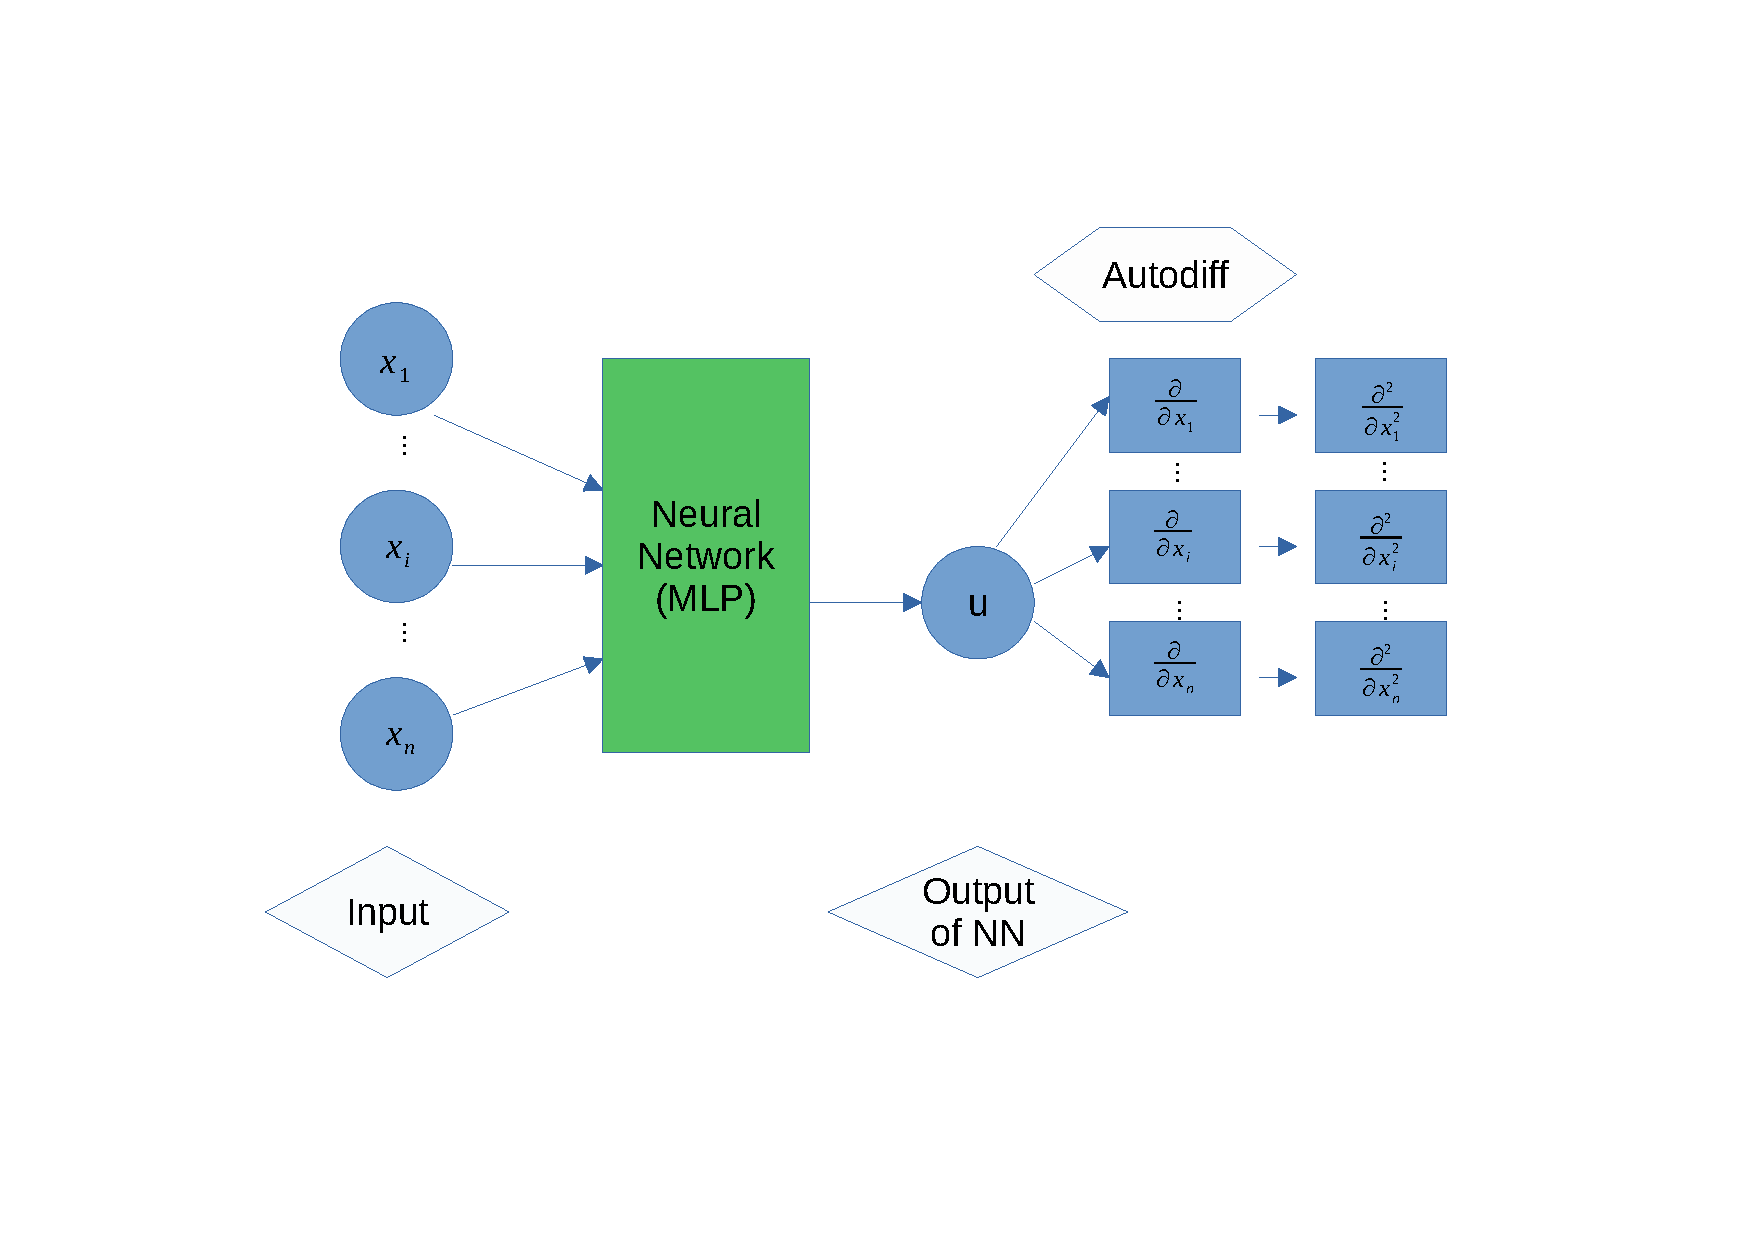
\includegraphics[width=15cm]{chapters/chapter1/pinn}
	\label{pinn}
	\caption{PINN model for Laplace Equation}
\end{figure}
In figure \ref{pinn} we can observe the architecture of such physics informed model. 
The Loss functions that we need to use to properly train our network are
\begin{eqnarray}
	\text{Loss}_s(\Theta) &=& \frac{1}{N}\sum^N_i\left(u_{\Theta}(\mathbf{x}_i)- u_i\right)^2,\\
	\text{Loss}_r(\Theta) &=& \frac{1}{R}\sum^R_i\left(\frac{\partial u_{\Theta}(\mathbf{x}_i)}{\partial x_i} - f(\mathbf{x}_i)\right)^2,\\
	\text{Loss}_l(\Theta) &=& \Delta u_{\Theta},\\
	\text{Loss}(\Theta) &=& \omega_s \text{Loss}_s +\omega_r \text{Loss}_r +\omega_l \text{Loss}_l .
\end{eqnarray}
The $\omega_s$,$\omega_r$,$\omega_l$, in this case are coefficients $0\leq \omega \leq 1$ and they are there to improve optimization capabilities which is defined as
\begin{equation}
	\Theta^* = \arg\min\text{Loss}(\Theta).
\end{equation}
The $\Theta$ are learnable parameters which can be updated with $\Theta^*$ trough optimization algorithm.\\
Such model wouldn't be possible without Automatic Differentiation\cite{} which are offered from machine learning library $\texttt{pytorch}$\cite{}. In this example we need big bunch of data and the optimization of the model could be very slow in addition if we don't have a computation capable hardware for it. Obtaining the data could be done only with exactly measurement or using some numerical solvers like FEM or Isogeometric Analysis. Don't forget, that there are Poission Equation, Wave Equation which are dependent on time $t$.\\
Those PDEs have mostly application in electrotechnical(Electro-magnetical fields) and  civil Engineering(static in construction).
In this thesis we won't work on the PDEs but similar to this topic we will try to train a model to predict the Dynamics of some physical phenomena and non-/holonomic systems of the robots.\\
The Dynamics for Robots are trivially defined as simple Second Level Ordinary Differential Equation\cite{} .
\begin{equation}
	\mathbf{M}\ddot{\mathbf{x}}(t) + \mathbf{D}(\dot{\mathbf{x}}(t)) + \mathbf{C}(\mathbf{x}(t))=0,
\end{equation} but there are other forms, as Langrange Equations of Motion if our system is holonomic\cite{}. It is based on Lagrange Function which is based on Kinetik $T$ and Potential $U$ Energy
\begin{eqnarray}
	\mathcal{L} &=& T - V,\\
	\frac{d}{dt}\frac{\partial \mathcal{L}}{\partial \dot{q}_i} - \frac{\partial \mathcal{L}}{\partial q_i}&=&0.
\end{eqnarray}   
The Lagrange Equations are used in Delan\cite{} Physics informed network and in simillar manner, but for us are most interesting to use Hamiltonian Equations of Motion.
They work for holonomic and non-holonomic systems and they are capable to build First Level Ordinary Equation
\begin{equation}
	\dot{x} = f(x,t)
\end{equation} \\
or in Hamiltonian Form where $\mathcal{H} = T + V$
\begin{equation}
	\dot{\mathbf{z}} = \mathbf{J}\frac{\partial\mathcal{H}}{\partial \mathbf{z}}
\end{equation} where $\mathbf{z}=[\mathbf{q},\mathbf{p}]^T$ and $\mathbf{J} = \begin{bmatrix}
0 & \mathbf{I}_n\\
-\mathbf{I}_n & 0
\end{bmatrix} $\\
\begin{figure}[h!]
	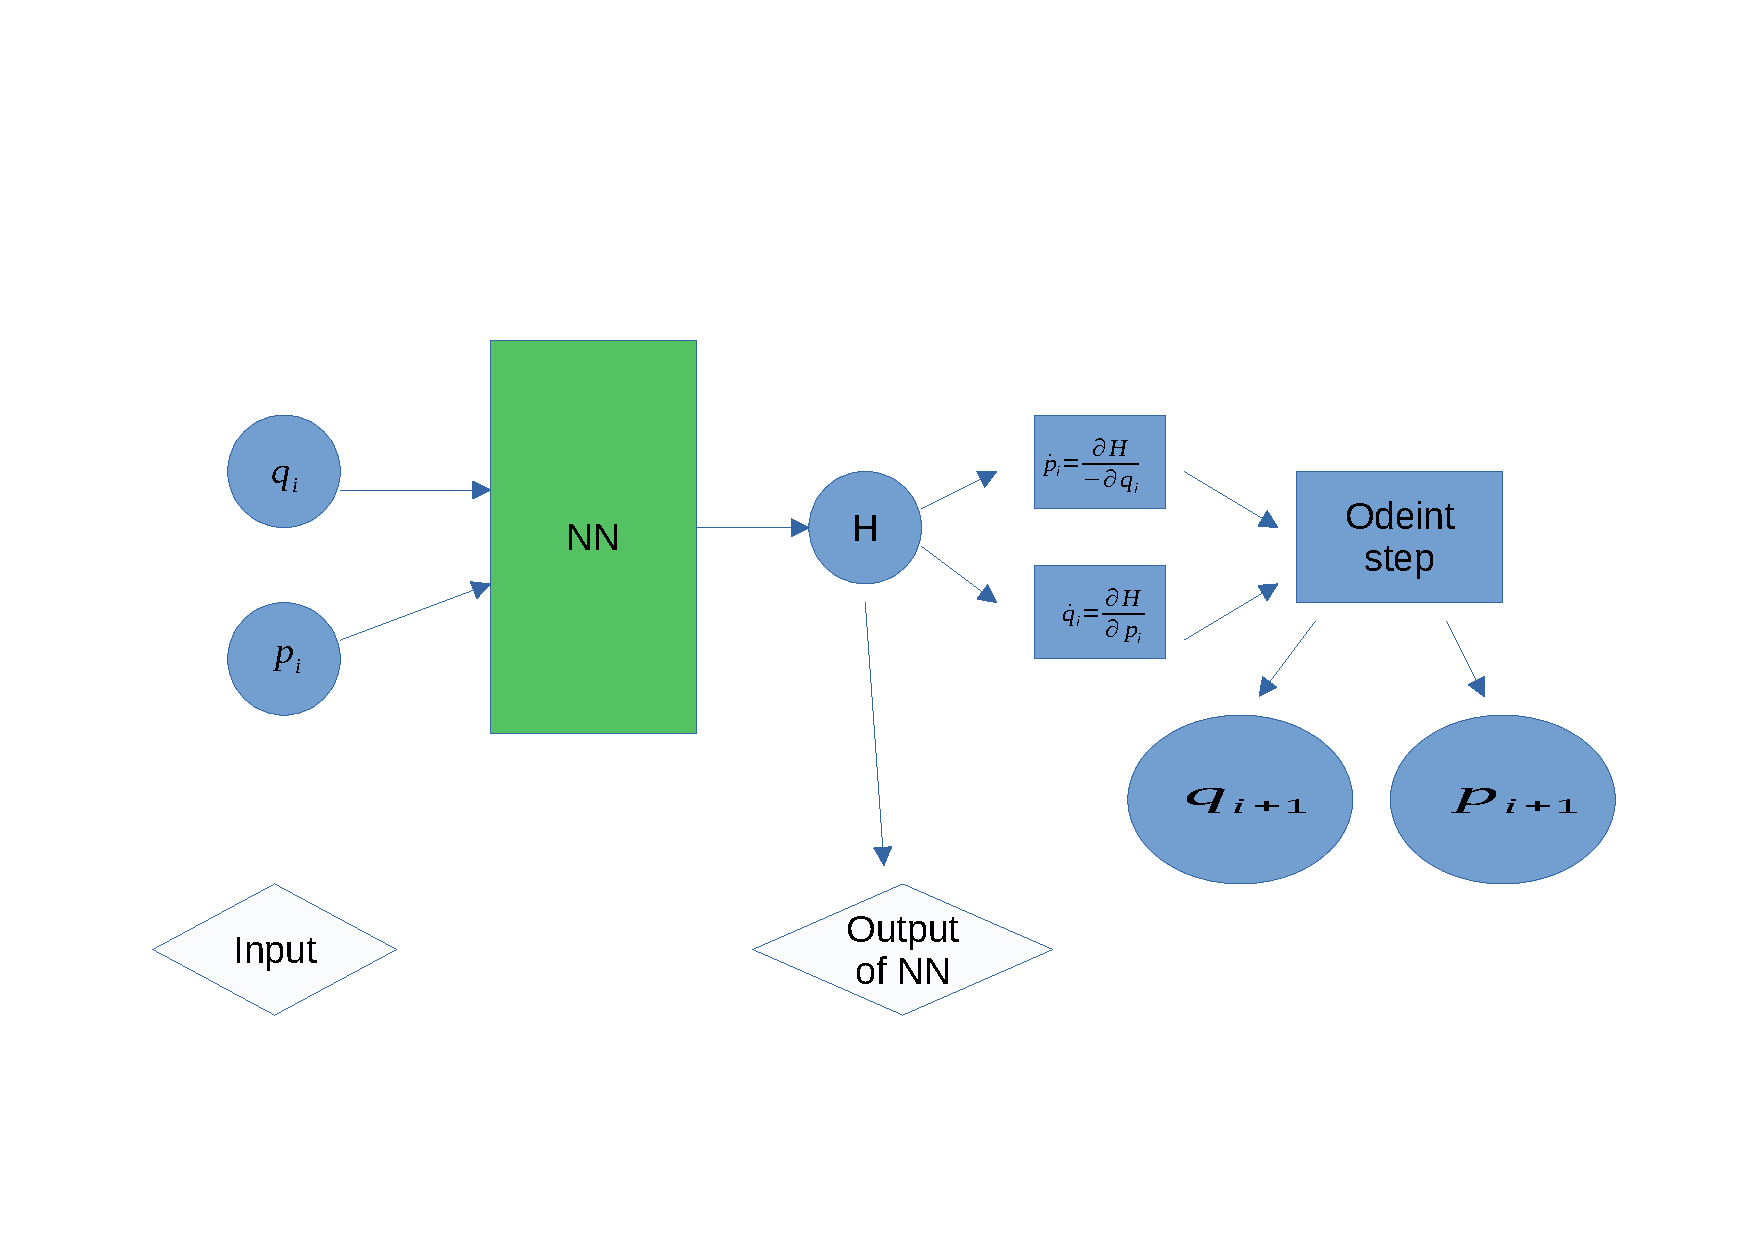
\includegraphics[width=15cm]{chapters/chapter1/hnn}
	\label{hnn}
	\caption{HNN model with integration solver step}
\end{figure}
One of such model is introduced in the \cite{} and it is called HNN. it architecture you can observe in figure \ref{hnn}.
We will make it more interesting introducing the Graph Neural Network and try to use it as a base of our architecture.\\
In this thesis we will discuss what are Hamiltonian equations and how to obtain them. In our research we stumbled upon the fact, that there are no quality datasets for training the Neural Networks which are based on physics. With this fact we brew 4 popular datasets which are based on Hamiltonian Equations of Motion.\\
Next we made new and revisit old neural architectures and test NeuralODE as new Nerual Paradigm into treaining the solutions of ODEs.\\
In the experiments we tested the capabilites of Graph Neural Networks, how do they adapt to diverse training data and their possibility to reduce or increase a degree of freedom in the training. For example how similar is the movement between 3 and 4 bodied pendulum on the same trained set of neural parameters. We hope that we will give the insight in those topics.    








%% related works, philosophy, motivations, my contributions
